\chapter{Вычислительные методы для теории представлений аффинных алгебр Ли}
\label{cha:computational-methods}

В данной главе мы описываем вычислительный пакет  {\bf Affine.m}, разработанный нами на основе идей и методов, изложенных в главах \ref{cha:affine-lie-algebras}, \ref{cha:BGG}. Этот пакет для популярной системы компьютерной алгебры {\it Mathematica} может использоваться для вычислений в теории представлений конечномерных и аффинных алгебр Ли. Реализованные в пакете алгоритмы основываются на свойствах весов и симметрии Вейля. Основные проблемы, которые может решать данный пакет -- это вычисление кратностей весов в неприводимых модулях и модулях Верма, построение правил ветвления и функций ветвления, а также разложение тензорных произведений. Такие задачи важны с точки зрения физических приложений (см. главы \ref{cha:CFT},\ref{sec:SLE}) и в данной главе мы приводим дополнительные примеры. 

Вычислительные методы в теории представлений имеют долгую историю \cite{belinfante1989survey}, существует большое количество программ и пакетов для вычислений, связанных с алгебрами Ли \cite{simplie}, \cite{vanleeuwen1994lsp}, \cite{stembridge1995mps,coxweyl}, \cite{fischbacher2002ilp}, \cite{Fuchs:1996dd}.

Большинство популярных программ \cite{simplie}, \cite{vanleeuwen1994lsp}, \cite{fischbacher2002ilp}, \cite{coxweyl} создано для изучения теории представлений простых конечномерных алгебр Ли. Здесь основные вычислительные задачи это:
\begin{enumerate}
\item Построение корневой системы, определяющей свойства алгебры Ли, в том числе коммутационные соотношения.
\item Перечисление элементов группы Вейля, необходимое ввиду симметрии корневой системы и характеров представлений относительно группы Вейля.
\item Вычисление кратностей весов, коэффициентов ветвления и слияния
\end{enumerate}
Существуют различные алгоритмы для решения этих задач \cite{moody1982fast}, \cite{stembridge2001computational}, \cite{belinfante1989survey}, \cite{casselman1994machine}.
Третья задача наиболее сложна с точки зрения вычислений. Существует два рекуррентных алгоритма, основывающихся на формуле Вейля для характеров и формуле Фрейденталя для кратностей. В данной главе мы их опишем.

Бесконечномерные алгебры Ли гораздо сложнее исследовать и число имеющихся программ гораздо меньше. 
Однако структура аффинных алгебр Ли позволяет адаптировать к ним вычислительные алгоритмы, предложенные для конечномерных алгебр Ли \cite{Fuchs:1996dd}, \cite{gannon2001algorithms}, \cite{kass1990ala}. В книге \cite{kass1990ala}, изданной в 1990 году, приведены таблицы кратностей весов неприводимых представлений и другие вычисленные характеристики аффинных алгебр и их модулей. Однако нам на данный момент не известны пакеты для популярных систем компьютерной алгебры, которые можно было бы использовать для воспроизведения и расширения этих результатов.

Чтобы исправить этот недостаток, нами был создан пакет {\bf Affine.m} для популярной системы  {\it Mathematica}. Возможности и ограничения этого пакета мы и описываем в этой главе. Кроме того, мы приводим некоторые примеры, связанные с физическими приложениями. 

Необходимые сведения из теории представлений приведены в главе \ref{cha:affine-lie-algebras}. Здесь мы начинаем с описания структур данных пакета  {\bf Affine.m}, использующихся для описания различных объектов теории представлений  (раздел \ref{sec:core-datastructures}), обсуждаем алгоритмы  (раздел \ref{sec:comp-algor}) и приводим примеры  (раздел \ref{sec:examples}). 

\section{Структуры данных}
\label{sec:core-datastructures} 
Хотя {\it Mathematica} -- нетипизированный язык программирования, в нем можно создавать структурированные объекты и проверять их типы используя сопоставление с шаблоном (pattern matching) \cite{shifrinmathematica}, \cite{maeder2000computer}.
\subsection{Веса}
\label{sec:weights}

Веса представляются двумя структурами данных: \lstinline{finiteWeight} для конечномерных алгебр Ли и \lstinline{affineWeight} для аффинных алгебр Ли.

Внутренняя структура веса конечномерной алгебры Ли представляет собой  \lstinline{List} с заголовком \lstinline{finiteWeight}, его компоненты -- это координаты веса в ортогональном базисе выбранном согласно Бурбаки \cite{bourbaki2002lie}.
Аффинный вес представляет собой расширение конечномерного веса с добавлением уровня и грейда. 

В пакете {\bf Affine.m} содержится набор функций для работы с весами конечномерных и аффинных алгебр Ли. Полный список доступен во встроенной справке пакета. Важнейшие из них -- это определение операций сложения, умножения на число и скалярного произведения (билинейной формы) для весов. В результате можно использовать традиционные обозначения при работе с  {\bf Affine.m}:
\begin{lstlisting}
  w=makeFiniteWeight[{1,0,3}];
  v=makeFiniteWeight[{3,2,1}];
  2*w+v==makeFiniteWeight[{5,2,7}]
  w.v==6
\end{lstlisting}

Использование ортогонального базиса во внутренней структуре весов позволяет нам работать с весами без полного задания корневой системы. Это полезно при изучении редукции на подалгебры, так как корни подалгебры можно задать вручную, путем указания их координат в ортогональном базисе.

\subsection{Корневые системы}
\label{sec:root-systems}

Чтобы задать конечномерную или аффинную алгебру достаточно определить ее корневую систему. Корневые системы представляются двумя структурами данных \lstinline{finiteRootSystem} и \lstinline{affineRootSystem}. Вторая структура является расширением первой. Мы предлагаем несколько конструкторов для этих структур данных. Во-первых, можно определить простое корни явно, например, при изучении вложения $B_2\subset B_4$ можно использовать определение
\begin{lstlisting}
  b2b4=makeFiniteRootSystem[ { {1,-1,0,0}, {0,1,0,0} } ]
\end{lstlisting}
Для корневых систем простых конечномерных алгебр Ли есть специальные конструкторы:
\begin{lstlisting}
  b2=makeSimpleRootSystem[B,2]
\end{lstlisting}
В графическом интерфейсе {\it Mathematica} можно использовать традиционные математические обозначения для простых алгебр Ли:


\begin{lstlisting}[mathescape=true]
  $B_2$ == makeFiniteRootSystem[ { {1, -1}, {0, 1} }]
\end{lstlisting}

Нескрученные аффинные корневые системы могут быть созданы как аффинные расширения корневых систем конечномерных алгебр Ли, например:
\begin{lstlisting}
  b2affine = makeAffineExtension[b2]
\end{lstlisting}
В графическом интерфейсе это же определение можно ввести просто как $\hat{B}_2$.

Полупростые алгебры Ли представляют собой прямые суммы простых:
\begin{lstlisting}[mathescape=true]
  $A_1\oplus A_1$ == finiteRootSystem[2, 2, {finiteWeight[2, {1, 0}], finiteWeight[2, {0, 1}]}]
\end{lstlisting}
%% The problem is here

Предикат \lstinline{rootSystemQ} проверяет, является ли объект корневой системой конечномерной или аффинной алгебры Ли.

Список простых корней -- это определяющее свойство корневой системы, поэтому он доступен как \lstinline{rs[simpleRoots]}.

В пакете реализовано несколько функций для основных характеристик корневой системы. Вектор Вейля дается функцией
\lstinline{rho[rs_?rootSystemQ]}:
\begin{lstlisting}[label=list:1]
  In[1]  =  rho[b2]
  Out[1]  =  finiteWeight[2, {3/2, 1/2}]
\end{lstlisting}
Положительные корни строятся функцией  \lstinline{positiveRoots[rs_?rootSystemQ]}. Для аффинной алгебры Ли эта и аналогичные функции возвращают список до некоторого фиксированного грейда. Это максимальное значение грейда задается как свойство \lstinline{rs[gradeLimit]} и по умолчанию равняется 10. Список корней  (вплоть до грейда \lstinline{gradeLimit}) строится функцией \lstinline{roots[rs]}. Матрица Картана и фундаментальные веса вычисляются функциями \lstinline{cartanMatrix} и \lstinline{fundamentalWeights} соответственно.

Вес алгебры Ли можно задать его индексами Дынкина
\begin{lstlisting}
  weight[b2][1,2] == makeFiniteWeight[{2, 1}]
\end{lstlisting}
Функция \lstinline{dynkinLabels[rs_?rootSystemQ][wg_?weightQ]} возвращает индексы Дынкина веса \lstinline{wg} по отношению к корневой системе \lstinline{rs}.

Элементы группы Вейля задаются номерами элементарных отражение, так что элемент  $w=s_{1}s_{2}s_{1}$ группы Вейля алгебры Ли $B_{2}$ строится вызовом функции \lstinline{weylGroupElement[b2][1,2,1]}. После этого его можно применить к весам:
\begin{lstlisting}
  w = weylGroupElement[b2][1,2,1];
  w @ makeFiniteWeight[{1,0}] == makeFiniteWeight[{-1,0}]
\end{lstlisting}

Вычисление лексикографически минимальной формы \cite{casselman1994machine,casselman1995automata} для элементов группы Вейля можно реализовать при помощи шаблонов в  {\it Mathematica}. В работе \cite{KallenShortlex} представлены правила подстановки на языке {\it Mathematica} для такого вычисления в случае простых конечномерных и аффинных алгебр Ли. Наше представление для элементов группы Вейля совместимо с кодом \cite{KallenShortlex}:
\begin{lstlisting}[mathescape=true]
  In[1]  = $<<$A3reduce;
           reduce[s[1,2,1,2,1,3,2,1,1]]
  Out[1] = s[2, 3, 2]

  In[2]  = (weylGroupElement[$A_{3}$] @@ reduce[s[1,2,1,2,1,3,2,1,1]]) @ weight[$A_{3}$][-1,-2,-1]
  Out[2] = finiteWeight[4, {-2, 2, 1, -1}]

  In[3]  = dynkinLabels[$A_{3}$][Out[2]]
  Out[3] = {-4, 1, 2}
\end{lstlisting}

\subsection{Формальные элементы}
\label{sec:formal-elements}

Формальные элементы представляются специальной структурой данных \lstinline{formalElement}. Эта структура данных представляет собой хэш-таблицу, реализованную через механизм \lstinline{DownValues}. Ключами в таблице выступают веса, стоящие в экспонентах формального элемента, а значениями -- соответствующие кратности.  Вызов \lstinline[mathescape=true]!makeFormalElement[{$\gamma_{1},\dots,\gamma_{n}$},{$m_{1},\dots,m_{n}$}]! создает структуру данных, представляющую элемент $\sum_{i=1}^{n} m_{i} e^{\gamma_{i}}$ формальной алгебры $\mathcal{E}$. Операции в алгебре  $\mathcal{E}$ реализованы для структуры \lstinline{formalElement}: формальные элементы можно складывать, умножать на число или экспоненту веса. Кроме того, есть умножение формальных элементов, но нет операции деления.
\begin{lstlisting}[mathescape=true]
  In[1]  = makeFormalElement[{makeFiniteWeight[{1,1}],makeFiniteWeight[{0,0}]},{1,2}] *
             (2 * Exp[makeFiniteWeight[{1,0}]] *
             makeFormalElement[{makeFiniteWeight[{1,1}],makeFiniteWeight[{0,0}]},{1,2}]);
  In[2]  = In[1][weights]
  Out[2] = {finiteWeight[2, {1, 0}], finiteWeight[2, {2, 1}], finiteWeight[2, {3, 2}]}

  In[3]  = In[1][multiplicities]
  Out[3] = {8, 8, 2}
\end{lstlisting}

\subsection{Модули}
\label{sec:modules}

{\bf Affine.m} можно использовать для изучения различных видов модулей, например, модулей Верма, неприводимых модулей и параболических модулей Верма. Для представления произвольного модуля используется структура данных  \lstinline{module}. 
Свойства модуля можно вывести из набора его сингулярных весов используя формулы Вейля для характеров \eqref{eq:11},\eqref{eq:12},\eqref{eq:18},\eqref{eq:13}. Множество сингулярных весов может обладать вейлевой симметрией. Это может быть симметрия по отношению к действию группы Вейля алгебры  $W_{\gf}$ или по отношению к действию группы Вейля некоторой подалгебры $W_{\af}$, как в случае параболических модулей Верма. В этом случае можно ограничиться изучением главной камеры Вейля $C_{\af}$. Чтобы воспользоваться такой симметрией общий конструктор для структуры данных \lstinline{module} принимает несколько параметров \lstinline{makeModule[rs_?rootSystemQ][singWeights_formalElement,subs_?rootSystemQ|emptyRootSystem[],limit:10}. Здесь \lstinline{rs} -- корневая система алгебры Ли $\gf$,\lstinline{singWeights} -- набор сингулярных весов,  \lstinline{subs} -- корневая система, соответствующая группе Вейля  $W_{\af}$, являющейся группой (анти-)симметрии множества сингулярных весов. Параметр \lstinline{limit} ограничивает вычисления в случае бесконечномерных модулей, таких, как модули Верма и параболические модули Верма.
Существует несколько специализированных конструкторов для различных типов модулей старшего веса:
\begin{lstlisting}[mathescape=true]
vm=makeVermaModule[$B_{2}$][{2,1}];
pm=makeParabolicVermaModule[$B_{2}$][weight[$B_{2}$][2,1],{1}];
im=makeIrreducibleModule[$B_{2}$][2,1];
GraphicsRow[textPlot/@{im,vm,pm}]
$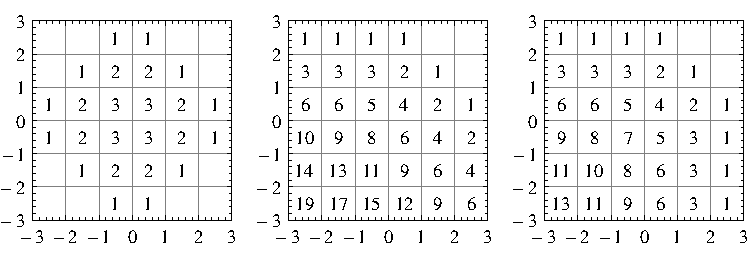
\includegraphics[width=130mm]{figures/irrep-verma-pverma}$
\end{lstlisting}

Как мы уже отмечали, свойства модулей определяются его сингулярным элементом. Функция  \lstinline{singularElement[m_module]} возвращает сингулярный элемент модуля в виде структуры данных  \lstinline{formalElement}. Характер  (вплоть до предела \lstinline{limit} для  (параболических) модулей Верма) вычисляется функцией \lstinline{character[m_module]}. Прямая сумма модулей является модулем и мы используем естественные обозначения
\begin{lstlisting}[mathescape=true]
im1=makeIrreducibleModule[$B_{2}$][weight[$B_{2}$][2,1]];
im2=makeIrreducibleModule[$B_{2}$][weight[$B_{2}$][1,2]];
textPlot[im1$\oplus$ im2]
$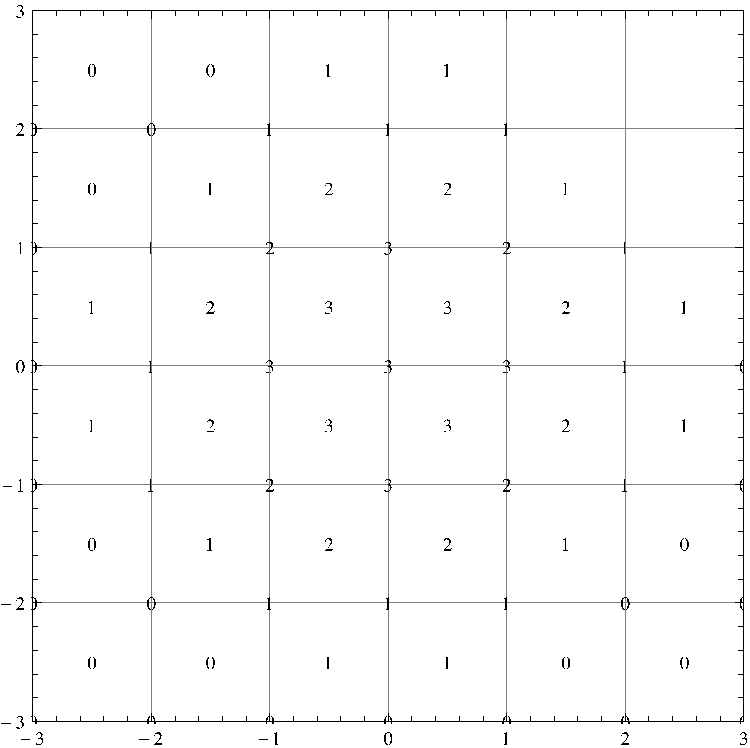
\includegraphics[width=60mm]{figures/irrep-sum}$
\end{lstlisting}

Тензорное произведение модулей тоже реализовано, но только для модулей конечномерных алгебр Ли. Это связано с тем, что тензорные произведения модулей аффинных алгебр Ли приводят к возникновению различных дополнительных структур  \cite{kazhdan1994tensor3,kazhdan1993tensor1,kazhdan1993tensor2}, изучение которых пока лежит за пределами наших интересов. 
\begin{lstlisting}[mathescape=true]
textPlot[makeIrreducibleModule[$A_{1}$][5]$\otimes$ makeIrreducibleModule[$A_{1}$][3]];
$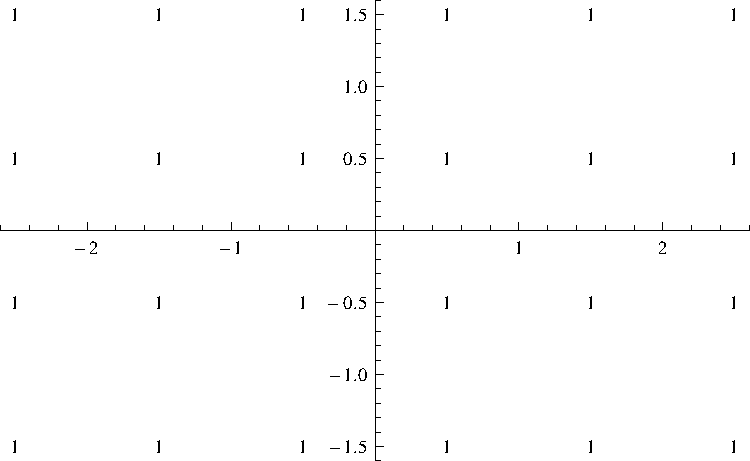
\includegraphics[width=60mm]{figures/tensor-product}$
\end{lstlisting}
\section{Основные алгоритмы}
\label{sec:comp-algor}
   
Существует два рекуррентных соотношения \eqref{eq:15}, \eqref{eq:14}, которые можно использовать для вычисления кратностей весов в неприводимых модулях. Оба алгоритма состоят из следующих шагов:
\begin{enumerate}
\item Построение списка весов в главной камере Вейля путем вычитания всех возможных комбинаций простых корней их старшего веса (например, для конечномерной алгебры вычитаем корень  $\alpha_{1}$ из старшего веса $\mu$ до тех пор, пока остаемся внутри  $\bar C$, затем вычитаем корень $\alpha_{2}$ из всех весов полученных на перво шаге и так далее).
\item Сортировка списка весов по значению их скалярного произведения с вектором Вейля.
\item Рекуррентное вычисление кратностей по формуле. Если вес, необходимый для вычислений оказывается вне главной камеры Вейля, то используется симметрия относительно группы Вейля.
\end{enumerate}
Различие в производительности алгоритмов происходит от количества предыдущих значений, требующихся для вычисления кратности веса. В случае рекуррентного соотношения, основанного на формуле Вейля  \eqref{eq:14} это количество постоянно и равно числу элементов в группе Вейля (если мы находимся далеко от внешнего контура диаграммы представления). При использовании формулы Фрейдентала \eqref{eq:15} требуемое число предыдущих значений растет с расстоянием от внешнего контура диаграммы представления.  Поэтому формула Фрейденталя работает быстрее, если вес близок к границе или ранг алгебры и размер группы Вейля велик \cite{moody1982fast}. Заметим, что формула Фрейденталя работает только для неприводимых модулей и не подходит для изучения (обобщенных) модулей Верма.

Мы осуществили тестирование производительности наших реализаций алгоритмов, основанных на формуле Фрейденталя и формуле \eqref{eq:15} и получили результаты, представленные на Рисунке  \ref{fig:freudenthal-racah-times}. Там показана зависимость времени вычислений от числа весов в модуле.

\begin{figure}[h]
  \noindent\centering{
    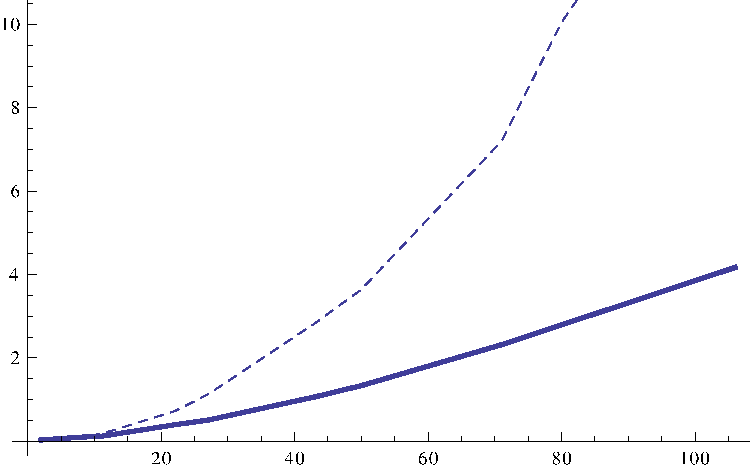
\includegraphics[width=80mm]{figures/timing}
  }
  \caption{Время работы алгоритмов, основанных на формуле Фрейденталя \eqref{eq:15} (пунктир) и рекуррентном соотношении \eqref{eq:14} (сплошная линия) в зависимости от количества весов в  $\bar C$ для вычисления кратностей в представлениях алгебры $B_{2}$.}
\label{fig:freudenthal-racah-times}

\end{figure}

При вычислении коэффициентов ветвления использование формулы Фрейденталя требует полного построения формальных характеров представления алгебры и всех представлений подалгебры, входящих в его разложение. Такой подход становится непрактичным для большого ранга алгебры и подалгебры, например, при максимальных вложениях. 

Альтернативный алгоритм описан в разделе \ref{sec:algorithm}. Рассмотренный там же пример регулярного вложения \ref{sec:someth-high-dimens}  $B_{2}\subset B_{4}$ позволяет сделать следующее сравнение числа требующихся операций. В данном примере веер вложения состоит из 24 элементов. Для разложения модуля алгебры  $B_{4}$ необходимо построить подмножество сингулярных весов модуля, проектирующихся в главную камеру Вейля подалгебры $B_{2}$. Полное множество сингулярных весов состоит из 384 элементов, в главную камеру Вейля проектируется не более 48, так что время на построение этого множества пренебрежимо мало, если число коэффициентов ветвления более 48. Мы можем оценить сверху общее число операций для вычисления коэффициентов ветвления произведением числа весов в главной камере Вейля подалгебры с ненулевыми коэффициентами ветвления на число элементов веера вложения. 
С другой стороны, при использовании алгоритма, основанного на построении всех характеров при помощи формулы Фрейденталя мы должны вычислить кратности для каждого модуля в разложении, так что общее количество операций растет с ростом числа весов в представлении быстрее, чем квадрат числа весов в главной камере Вейля подалгебры с ненулевыми коэффициентами ветвления. 

Чтобы проиллюстрировать эту разницу в производительности алгоритмов, мы приводим Рисунок \ref{fig:branching}, на котором показано время, необходимое для вычисления коэффициентов ветвления для вложения $B_{3}\subset B_{4}$.

\begin{figure}[h]
  \noindent\centering{
   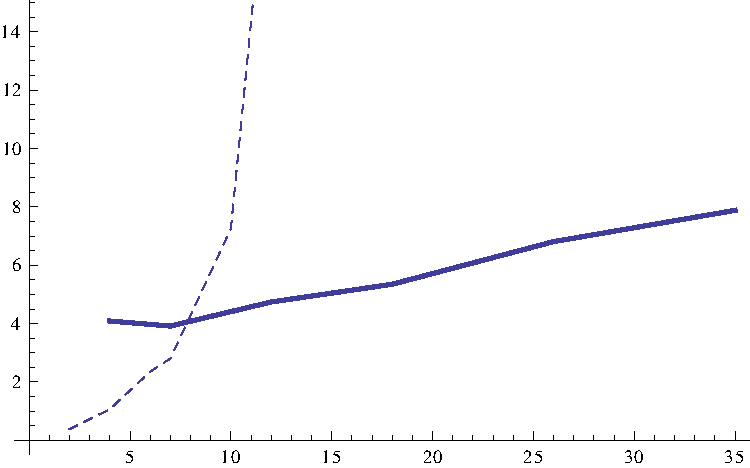
\includegraphics[width=100mm]{figures/branching-timing}
  }
  \caption{Время работы алгоритмов, основанных на применении формулы Фрейденталя \eqref{eq:15} (пунктиром)  и рекуррентного соотношения \eqref{recurrent-rel} (сплошная линия) с ростом числа весов в  $\bar C$ при вычислении коэффициентов ветвления для вложения $B_{3}\subset B_{4}$.}
  \label{fig:branching}
\end{figure}

\section{Примеры}
\label{sec:examples}
В этом разделе мы приводим примеры вычислений, проведенных с использованием {\bf Affine.m} и код, который для этого потребовался.

\subsection{Разложение тензорных произведений модулей конечномерных алгебр Ли на неприводимые}
\label{sec:tens-prod-decomp}

Вычисление коэффициентов слияния для разложения тензорного произведения модулей старшего веса в прямую сумму неприводимых модулей важно для различных приложений в физике. Например, мы можем рассматривать спин составной системы, такой как атом. Другой интересный пример -- это интегрируемые спиновые цепочки, состоящие из  $N$ частиц со спинами, живущими в некотором представлении  $L$ алгебры Ли $\gf$, с  $\gf$-инвариантным гамильтонианом $H$, описывающим спин-спиновое взаимодействие ближайших соседей. Чтобы решить такую систему, то есть найти собственные состояния гамильтониана, мы должны разложить  $L^{\otimes N}$ в прямую сумму неприводимых $\gf$-модулей меньшей размерности и диагонализовывать гамильтониан на этих модулях.

Для фундаментальных представлений простых алгебр Ли иногда можно написать аналитический ответ, описывающий зависимость коэффициентов разложения от  $N$ (См. работу \cite{LyakhovskyPostnova2011}). Наш код позволяет получать численные ответы, которые можно использовать для проверки этих аналитических результатов.

Рассмотрим тензорную степень $\left(L^{[1,0]}\right)^{\otimes 4}$ первого фундаментального представления алгебры $B_{2}$. Коэффициенты разложения тензорной степени на неприводимые модули -- это коэффициенты ветвления модуля алгебры $B_{2}\oplus B_{2}\oplus B_{2}\oplus B_{2}$ на диагональную подалгебру $B_{2}\subset B_{2}\oplus B_{2}\oplus B_{2}\oplus B_{2}$. Следующий код осуществляет необходимые вычисления:
\begin{lstlisting}[mathescape=true]
fm = makeIrreducibleModule[$B_{2}$][1, 0];
tp = ((fm$\otimes$ ]fm)$\otimes$ fm)$\otimes$]fm;
subs = makeFiniteRootSystem[
  {1/4*{1, -1, 1, -1, 1, -1, 1, -1}, 
   1/4*{0, 1, 0, 1, 0, 1, 0, 1}}];
bc = branching[tp, subs];
{bc[#], dynkinLabels[subs][#]} & /@ bc[weights]
\end{lstlisting}
Он выдает в результате следующий набор старших весов и коэффициентов разложения:
\begin{lstlisting}
{{1, {4, 0}}, {3, {2, 2}}, {0, {3, 0}}, 
{2, {0, 4}}, {3, {1, 2}}, {6, {2, 0}}, 
{6, {0, 2}}, {1, {1, 0}}, {3, {0, 0}}}]
\end{lstlisting}

Возвращаясь к проблеме диагонализации гамильтониана спиновой цепочке, мы можем заметить, что вместо диагонализации оператора в пространстве размерности  $625$ мы можем диагонализовывать операторы в пространствах размерностей $55, 81, 30, 35, 35, 14, 10, 5, 1$.

\subsection{Ветвления и параболические модули Верма}
\label{sec:branch-parab-verma}

Мы иллюстрируем обобщенную резольвенту Бернштейна-Гельфанда-Гельфанда (см. главу \ref{cha:BGG}) диаграммами параболических модулей Верма алгебры $G_{2}$, возникающих в разложении неприводимого модуля $L^{[1,1]}_{G_{2}}$:
\begin{equation}
\mathrm{ch}\left( L^{\mu }\right) =\sum_{u\in U}\;e^{\mu _{\aft}\left(
u\right) }\epsilon (u)\mathrm{ch}M_{I}^{\mu _{\frak{a}_{\perp }}\left(
u\right) }.  \label{char-in-gen-verma-mod}
\end{equation}
Характер  $L^{[1,1]}$ представлен на Рисунке \ref{branching-bgg}, характеры обобщенных модулей Верма в разложении  \eqref{char-in-gen-verma-mod} показаны на Рисунке  \ref{g2-pverma}. Характеры в верхнем ряду входят в формулу \eqref{char-in-gen-verma-mod} со знаком плюс, в нижнем -- со знаком минус. 


\begin{figure}[h]
  \noindent\centering{
    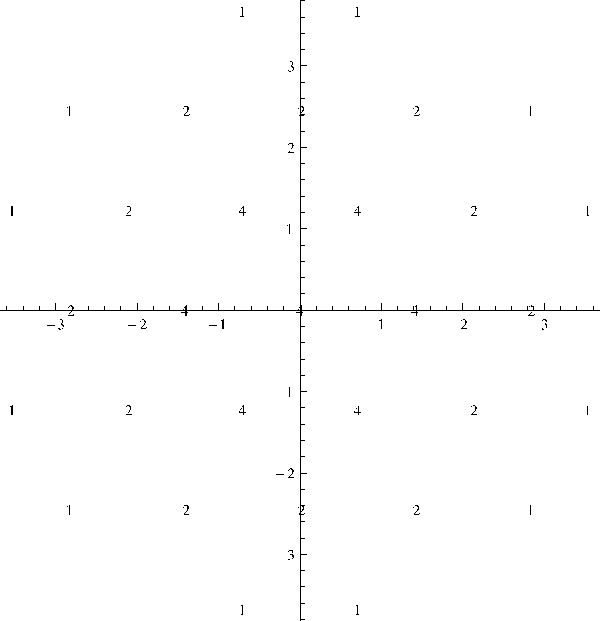
\includegraphics[width=80mm]{figures/G2-irrep}
  }
  \caption{Характер неприводимого модуля  $L^{[1,1]}$ алгебры $G_{2}$}
  \label{branching-bgg}
\end{figure}
\begin{figure}[h]
  \noindent\centering{
    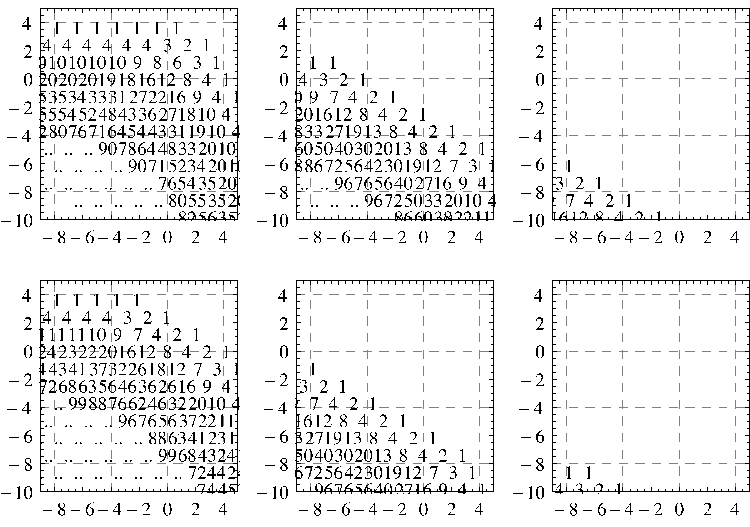
\includegraphics[width=150mm]{figures/G2-pverma}
  }
  \caption{Характеры обобщенных модулей Верма алгебры $G_{2}$, входящие в разложение характера $L^{[1,1]}$. Параболические модули Верма в верхнем ряду входят в разложение со знаком плюс, в нижнем -- со знаком минус.}
  \label{g2-pverma}
\end{figure}

\subsection{Струнные функции аффинных алгебр Ли и модели конформной теории поля}
\label{sec:string-funct-affine}
Струнные функции можно использовать для описания формальных характеров представлений старшего веса аффинных алгебр Ли. Эти функции обладают интересными аналитическими и модулярными свойствами \cite{kac1990idl,kac1988modular,kac1984infinite}.

{\bf Affine.m} позволяет вычислять степенное разложение для струнных функций. Рассмотрим аффинную алгебру Ли $\hat{sl(3)}=\hat A_{2}$ и ее модуль старшего веса $L^{(1,0,0)}$. Чтобы получить струнные функции используем следующий код:
\begin{lstlisting}[mathescape=true]
stringFunctions[$\hat A_2$,{1,1,2}]
{{0, 0, 4}, 
  $2 q + 10 q^2 + 40 q^3 + 133 q^4 + 398 q^5 + 1084 q^6 + 2760 q^7 + 6632 q^8 + 15214 q^9 + 33508 q^{10}$}, 
{{0, 3, 1}, 
  $2 q + 12 q^2 + 49 q^3 + 166 q^4 + 494 q^5 + 1340 q^6 + 3387 q^7 + 8086 q^8 + 18415 q^9 + 40302 q^{10}$}, 
{{1, 1, 2}, 
  $1 + 6 q + 27 q^2 + 96 q^3 + 298 q^4 + 836 q^5 + 2173 q^6 + 5310 q^7 + 12341 q^8 + 27486 q^9 + 59029 q^{10}$}, 
{{2, 2, 0}, 
  $1 + 8 q + 35 q^2 + 124 q^3 + 379 q^4 + 1052 q^5 + 2700 q^6 + 6536 q^7 + 15047 q^8 + 33248 q^9 + 70877 q^{10}$}, 
{{3, 0, 1}, 
  $2 + 12 q + 49 q^2 + 166 q^3 + 494 q^4 + 1340 q^5 + 3387 q^6 + 8086 q^7 + 18415 q^8 + 40302 q^9 + 85226 q^{10}$}
\end{lstlisting}
Аналогично для аффинной алгебры Ли $\hat G_{2}$ получаем
\begin{lstlisting}[mathescape=true]
stringFunctions[$\hat G_2$,{1,1,0}]
{{2, 0, 0}, 
  $1 + 8 q + 37 q^2 + 138 q^3 + 431 q^4 + 1227 q^5 + 3208 q^6 + 7901 q^7$}, 
{{0, 0, 1}, 
  $3 q + 18 q^2 + 73 q^3 + 247 q^4 + 736 q^5 + 2000 q^6 + 5070 q^7$}, 
{{1, 1, 0},
  $1 + 7 q + 32 q^2 + 117 q^3 + 370 q^4 + 1055 q^5 + 2780 q^6 + 6880 q^7$}, 
{{0, 2, 0}, 
  $3 q + 15 q^2 + 63 q^3 + 210 q^4 + 633 q^5 + 1725 q^6 + 4407 q^7$}
\end{lstlisting}

\subsection{Функции ветвления и  coset-модели конформной теории поля}
\label{sec:branch-funct-coset}

Считается, что рациональные модели конформной теории поля могут быть получены как  $G/A$ coset-модели, соответствующие вложениям $\af\subset\gf$. Эти модели можно реализовать как калибровочные теории  \cite{Hwang:1994yr, hwang1993brst} (см. раздел \ref{sec:coset-models-cft}). 

Функции ветвления для вложения  $\af\subset\gf$ являются статсуммами для моделей конформной теории поля на торе (см. \cite{difrancesco1997cft}).

В качестве первого примера мы демонстрируем вычисление функций ветвления для вложения $\hat A_{1}\to \hat B_{2}$ до десятого грейда:
\begin{lstlisting}[mathescape=true]
branchingFunctions[$\hat B_{2}$,makeAffineExtension[makeFiniteRootSystem[{{1, 1}}]], {1, 1, 1}]

 {{3, 0}, 
  $2 + 14 q + 52 q^2 + 154 q^3 + 410 q^4 + 994 q^5 + 2248 q^6 + 4832 q^7 + 9934 q^8 + 19680 q^9 + 37802 q^{10}$},
 {{2, 1}, 
  $4 + 20 q + 72 q^2 + 220 q^3 + 584 q^4 + 1424 q^5 + 3248 q^6 + 7012 q^7 + 14488 q^8 + 28844 q^9 + 55616 q^{10}$},
 {{0, 3}, 
  $4 q + 20 q^2 + 68 q^3 + 200 q^4 + 516 q^5 + 1224 q^6 + 2736 q^7 + 5808 q^8 + 11820 q^9 + 23236 q^{10}$},
 {{1, 2}, 
  $2 + 14 q + 54 q^2 + 168 q^3 + 462 q^4 + 1148 q^5 + 2656 q^6 + 5812 q^7 + 12130 q^8 + 24358 q^9 + 47328 q^{10}$}
\end{lstlisting}

Второй пример -- это вычисление функций ветвления для регулярного вложения  $\hat B_{2}\subset \hat C_{3}$:
\begin{lstlisting}[mathescape=true]
sub=makeAffineExtension[parabolicSubalgebra[$C_{3}$][2,3]];
branchingFunctions[$\hat C_{3}$,sub, {2, 0, 0, 0}]

{{0, 1, 0}, 
  $2 q - 20 q^3 + 24 q^4 + 82 q^5 - 320 q^6 + 108 q^7$}, 
{{1, 0, 0}, 
  $1 - q - 8 q^2 + 19 q^3 + 16 q^4 - 156 q^5 + 205 q^6 + 640 q^7$}, 
{{0, 0, 1}, 
  $q - 5 q^3 + 7 q^5$}
\end{lstlisting}

\section{Заключение}
\label{sec:conclusion}
В данной главе мы представили пакет {\bf Affine.m} для вычислений в теории представлений конечномерных и аффинных алгебр Ли. Он может использоваться для изучения групп Вейля, корневых систем, неприводимых модулей, модулей Верма и параболических модулей Верма конечномерных и аффинных алгебр Ли. Кроме того, мы обсудили основные идеи в реализации пакета  {\bf Affine.m}. 

Мы показали, что рекуррентный подход, основанный на формуле Вейля для характеров полезен не только для вычислений, но и позволяет прояснить связь с (обобщенной) резольвентой Бернштейна-Гельфанда-Гельфанда.

Также мы представили примеры вычислений с применением нашего пакета, полезных для различных физических и математических проблем. 

В следующих версиях программы мы планируем реализовать работу со скрученными аффинными алгебрами Ли, расширенными аффинными алгебрами и реализовать более полную поддержку вычислений коэффициентов разложения тензорных произведений.

\appendix

\section{Описание пакета}
\label{package}
Пакет может быть бесплатно загружен с сайта \url{http://github.com/naa/Affine}. Чтобы получить разрабатываемую версию кода можно использовать систему управления версиями {\it git} и команду
\begin{lstlisting}[language=bash]
 git clone git://github.com/naa/Affine.git
\end{lstlisting}

Содержимое пакета:
\begin{verbatim}
    Affine/                              Корневой каталог
      demo/                               Демонстрации
        demo.nb                                Демонстрационный файл
        paper.nb                               Код, содержащийся в статье 
      doc/                                 Каталог документации
        figures/                             рисунки в статье
          timing.pdf                           диаграмма, показывающая производительность
          branching-timing.pdf                 ...  для коэффициентов ветвления
          irrep-sum.pdf                        сумма неприводимых представлений B2
          irrep-verma-pverma.pdf               неприводимое представлений, модуль Верма и обобщенный модуль Верма для B2
          G2-irrep.pdf                         неприводимое представление G2
          G2-pverma.pdf                        параболический модуль Верма для G2
          tensor-product.pdf                   тензорное произведение модулей  A1
        bibliography.bib                     Библиографическая база
        paper.pdf                            Статья, описывающая пакет
        paper.tex                            Исходный LaTeX-файл статьи
        TODO.org                             Список доработок
      src/                                 Каталог исходного кода
        affine.m                             основной пакет
      tests/                               Каталог тестов
        tests.m                              тесты
      README.markdown                    Инструкция по установке и использованию
\end{verbatim}


%% References
%%
%% Following citation commands can be used in the body text:
%% Usage of \cite is as follows:
%%   \cite{key}         ==>>  [#]
%%   \cite[chap. 2]{key} ==>> [#, chap. 2]
%%

%% References with bibTeX database:

  %   \section*{References}
  %   \label{sec:references}
  %   
  %   
  %   \bibliography{bibliography}
  %   \bibliographystyle{phcpc}
  %   %\bibliographystyle{model1-num-names}
  %   
  %   
  %   %% Authors are advised to submit their bibtex database files. They are
  %   %% requested to list a bibtex style file in the manuscript if they do
  %   %% not want to use elsarticle-num.bst.
  %   
  %   %% References without bibTeX database:
  %   
  %   % \begin{thebibliography}{00}
  %   
  %   %% \bibitem must have the following form:
  %   %%   \bibitem{key}...
  %   %%
  %   
  %   % \bibitem{}
  %   
  %   % \end{thebibliography}
  %   
  %   
  %   

%%
%% End of file
%%% Local Variables: 
%%% mode: latex
%%% TeX-master: "thesis"
%%% End: 
